%\textcolor{red}{
In this section, we present our proposed \namekey{}, a robust symmetric key sharing between {\tt S} and each entity on $\Psi$, which allows different entities to obtain correct keys so that it can perform correct localization. % of \name{}. %\namekey{} is well employed to achieve shared keys setup and distribution in the initial period of \name{}, which promotes the robustness of fault localization for source and path verification.} 
Similar to DRKey \cite{kim2014lightweight}, \namekey{} provides the stateless operation on routers and enables each router not to store the symmetric keys. More especially, it also offers robustness against the interference of misbehaving entities. Fig. \ref{askeyfigure} shows how \namekey{} works when each entity creates the symmetric key and shares it with {\tt S}.
\vspace{-0.1in}
\subsection{ReqKey transmission from {\tt S} to {\tt D}}
\label{reqkeytransmission}
\begin{figure}%[H]
\begin{center}
  % Requires \usepackage{graphicx}
\includegraphics[width=8.3cm]{visio/laskey3.eps}
\caption{\namekey{} for symmetric key distribution with $\Psi$\emph{=}$\langle$\emph{S, R}$_1$\emph{,}$\cdots$\emph{R}$_\emph{n}$\emph{, D}$\rangle$, where \emph{R}$_{\emph{n+}1}$ is regarded as the destination {\tt D}.}\label{askeyfigure}
\end{center}
\vspace{-3mm}
\end{figure}
To achieve sharing symmetric keys with other entities, {\tt S} initializes ReqKey packet and %, which is then forwarded 
delivers it to {\tt D} through $\Psi$.
%At the beginning, ReqKey packet is firstly initialized by {\tt S} and then forwarded through $\Psi$ to {\tt D}. 
ReqKey contains $\Psi$, session identifier \emph{SessionID}, the public key set \emph{PubK} of all entities on $\Psi$ and {\tt S}'s signature \emph{Sign}$_\emph{S}$, as Eq. \ref{reqkeyfomat} shows.
\begin{equation}\label{reqkeyfomat}
\emph{ReqKey} =~ \{\Psi, \emph{SessionID}, \emph{PubK}, \emph{Sign}_\emph{S}\},
%\vspace{-0.06in}
\end{equation}
\noindent where \emph{SessionID} is the session identifier that is the hash over end-hosts' public keys (\emph{K}$_\emph{S}$ and \emph{K}$_\emph{D}$) and session's start time \emph{T}$_\emph{start}$. It can be computed by the following equation:
\begin{equation}\label{sessionidkey}
\emph{SessionID} = H(\emph{K}_\emph{S}\vert \vert \emph{K}_\emph{D}\vert \vert \emph{T}_{\emph{start}}).
\end{equation}
As Eq. \ref{signaturesource} shows, \emph{Sign}$_\emph{S}$ uses the destination address ({\tt D}) as one of the inputs, contributing to defending against ReqKey redirection or hijacking by modifying the destination address of ReqKey packet. %For example, if a misbehaved router redirects or hijacks \emph{ReqKey}, the downstream routers can drop this packet as the failed verification for \emph{Sign}$_\emph{S}$.
Certainly, \emph{Sign}$_\emph{S}$ is also keyed with \emph{K}$_\emph{S}^{\emph{-}1}$ that makes ReqKey away from source spoofing.
\begin{equation}\label{signaturesource}
\emph{Sign}_\emph{S} = \emph{Sign}_{\emph{K}^{\emph{-}1}_\emph{S}}H({\tt D}\vert \vert \Psi \vert \vert \emph{SessionID} \vert \vert \emph{PubK}).
\end{equation}

In addition to checking \emph{Sign}$_{\emph{S}}$, each intermediate entity \emph{R}$_\emph{i}$ creates and temporarily stores the symmetric key \emph{K}$_{\emph{S,R}_\emph{i}}$, which is calculated using pseudo-random function (PRF) keyed by local secret information (\emph{LSI}$_\emph{i}$), only known by \emph{R}$_\emph{i}$ (see Eq. \ref{ksri}).
\begin{equation}\label{ksri}
\emph{K}_{\emph{S}, \emph{R}_\emph{i}} = \emph{PRF}_{\emph{LSI}_\emph{i}}(\emph{SessionID} \vert \vert {\tt S}).
\end{equation}
\emph{R}$_\emph{i}$ starts the timer $\mathcal{T}_\emph{i}$ when ReqKey is delivered to the downstream entity, where $\mathcal{T}_\emph{i}$ is the timer maintained on \emph{R}$_\emph{i}$. 
%The \textbf{\emph{timer}} $\mathcal{T}_\emph{S}$ and $\mathcal{T}_\emph{i}$ are running on {\tt S} and \emph{R}$_\emph{i}$ on $\Psi$, respectively. 
It starts when the request package arrives and expires after a certain timeout, called \emph{\textbf{timer threshold}} that can be obtained by a \emph{round-trip time} (RTT). 
 %, and the temporary storage time of \emph{K}$_{\emph{S,R}_\emph{i}}$ relies on timer threshold. Unlike DRKey, our proposed \emph{LASKey} enable each router not have to insert the encrypted key into request packet, avoiding the risk of modification, discarding and redirection of the encrypted keys. Instead,
The created key \emph{K}$_{\emph{S,R}_\emph{i}}$ is temporarily stored until AckKey (detailed shortly) comes or $\mathcal{T}_\emph{i}$ expires. More considerately, \namekey{} makes each entity temporarily record the TTL value \emph{ttl}$_\emph{i}^\emph{r}$ of received ReqKey, which helps to avoid TTL attack.
\vspace{-0.1in}
\subsection{AckKey Transmission from {\tt D} to {\tt S}}
\label{ackkeytransmission}
To reply ReqKey, AckKey is initialized by {\tt D} and then sent back through intermediate entities towards {\tt S}, whose construction is as Eq. \ref{ackkeyformat} shows.
\begin{equation}\label{ackkeyformat}
\emph{AckKey} =~ \{\emph{ReqKey}, \emph{EncK}_{\emph{S,D}}, \emph{SignK}_\emph{D}\}.
%\vspace{-0.06in}
\end{equation}
\noindent
$\emph{EncK}_{\emph{S,D}}$ and $\emph{SignK}_\emph{D}$ are the encrypted \emph{K}$_{\emph{S},\emph{D}}$ and {\tt D}'s signature, respectively (detailed in Fig. \ref{askeyfigure}).\\
\indent
During AckKey's transmission, each entity adds its encrypted symmetric key \emph{EncK}$_{\emph{S,R}_\emph{i}}$ and signature \emph{SignK}$_{\emph{R}_\emph{i}}$ into AckKey. Note that when computing the signature \emph{SignK}$_{\emph{R}_\emph{i}}$, the encrypted symmetric keys and signatures of downstream entities (i.e., \emph{R}$_{\emph{i+}1}$,$\cdots$,\emph{R}$_\emph{D}$) will also be added as the input. In this case, each router \emph{R}$_\emph{i}$ only checks the \emph{SignK}$_{\emph{R}_{\emph{i+}1}}$ of its 1-hop downstream \emph{R}$_{\emph{i+}1}$, which can also defend against frame attack. Therefore, AckKey has the following construction (Eq. \ref{ackkeyformati}) when it arrives at \emph{R}$_\emph{i}$:\\
\begin{equation}\label{ackkeyformati}
\emph{AckKey} =~ \{\emph{ReqKey}, \emph{EncKset}_{\emph{i}}, \emph{SignKset}_\emph{i}, \emph{SignK}_{\emph{S},\emph{R}_\emph{i}}\},
%\vspace{-0.06in}
\end{equation}
\noindent where \emph{EncKset}$_\emph{i}$ and \emph{SignKset}$_\emph{i}$ are the sets of encrypted symmetric keys and signatures, respectively. Thus, AckKey can record the encrypted symmetric keys of all entities when it arrives at {\tt S}, as case \uppercase\expandafter{\romannumeral1} in Fig. \ref{disburbacktransmission} shows.\\
\indent To deal with the malicious discarding of either ReqKey or AckKey packet by the misbehaved entity, each entity (including {\tt S}) starts the timer $\mathcal{T}_\emph{i}$ when ReqKey passes through. If $\mathcal{T}_\emph{i}$ expires, i.e., \emph{R}$_\emph{i}$ does not receive AckKey within timer threshold, \emph{R}$_\emph{i}$ initializes a new AckKey, which contains \emph{EncK}$_{\emph{S,K}_{\emph{R}_\emph{i}}}$ and \emph{Sign}$_{\emph{K}_{\emph{R}_\emph{i}}}$. Thus, if any misbehaved entity drops ReqKey or AckKey, its upstream entity close to {\tt S} will forward their encrypted keys and signatures to {\tt S}. This is as case \uppercase\expandafter{\romannumeral2} in Fig. \ref{disburbacktransmission} shows, where the misbehaved entity \emph{R}$_\emph{3}$ can modify, drop and redirect ReqKey or AckKey packet for disturbing {\tt S}'s obtaining all entities' sampling information.
In this case, {\tt S} can achieve the fault localization to identify the misbehaved entity (described shortly). To avoid TTL attack, we use TTL values of both received ReqKey and AckKey as the input to compute \emph{SignK}$_{\emph{R}_\emph{i}}$. When AckKey is verified at each hop, \emph{R}$_\emph{i}$ obtains purposed TTL value of ReqKey and AckKey of other entities based on $\Psi$, and then use them to check others' signatures. If the misbehaved entity launches TTL attack, the signatures of its downstream entities will not be verified successfully.
%In \emph{LASKey} mechanism, a timer $\mathcal{T}$ is established on each node, which can defend against the discarding of \emph{ReqKey} and \emph{AckKey}. If the misbehaved router (say, \emph{R}$_\tau$) drops \emph{ReqKey} and \emph{AckKey} to disturb symmetric key distribution, the timer $\mathcal{T}_{\tau\emph{-}1}$ of its upstream router \emph{R}$_{\tau\emph{-}1}$ will expires, resulting in the transmission of its encrypted symmetric key and signature back to \emph{S}. Thus, if the discarding of \emph{ReqKey} or \emph{AckKey} occurs, \emph{S} can locate the misbehaved node according to the received \emph{AckKey} packet.
\begin{figure}%[H]
\begin{center}
  % Requires \usepackage{graphicx}
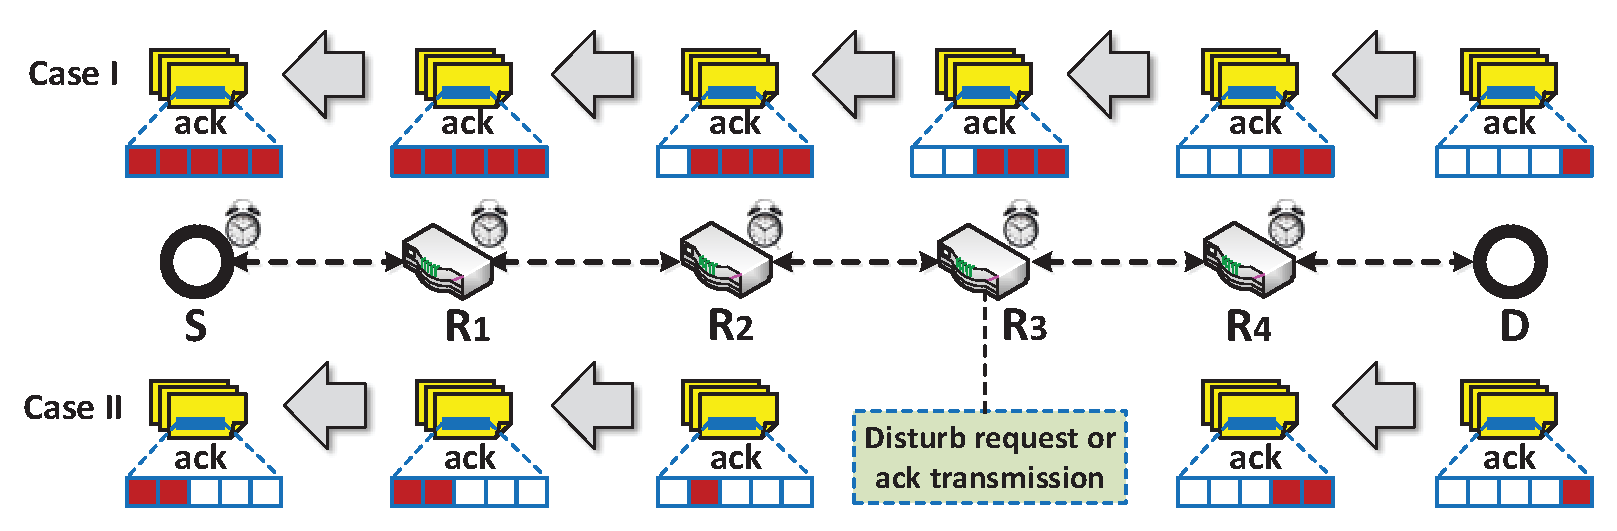
\includegraphics[width=1\columnwidth]{visio/disturbacktransmission.eps}
\caption{\namekey{} can ensure the robustness of symmetric keys distribution even facing unreliable communication channels. The red rectangle represents the ack of each network entity. Case \uppercase\expandafter{\romannumeral1} shows the AckKey packet can be securely delivered to {\tt S}, while case \uppercase\expandafter{\romannumeral2} depicts the misbehaved entity \emph{R}$_\emph{3}$ can interfere with ReqKey or AckKey packet transmission.}\label{disburbacktransmission}
\end{center}
\vspace{-3mm}
\end{figure}
\vspace{-0.1in}
\subsection{Symmetric Key Acquisition}
\label{keyacquisition}
The source {\tt S} needs to retrieve the symmetric keys shared with other entities on $\Psi$, which can be used to perform packet forwarding verification and fault localization.
In \name{}, {\tt S} can obtain symmetric keys from the received AckKey packet. Concretely, once receiving the AckKey packet, {\tt S} firstly checks the signatures and decrypts the encrypted keys to obtain the symmetric keys. Concretely, for each entity from \emph{R}$_1$ to {\tt D} on $\Psi$, if its signature is verified successfully using its public key, {\tt S} can obtain the symmetric key by decrypting the encrypted key using {\tt S}'s private key. In this way, the symmetric key set (denoted by $\mathbb{L}$) can be obtained:
\begin{equation}\label{symmetrickeyset}
\mathbb{L} ~\emph{=} ~\left \langle \emph{K}_{\emph{S},\emph{R}_1}, \emph{K}_{\emph{S},\emph{R}_2}, \cdots, \emph{K}_{\emph{S},\emph{D}} \right \rangle.
%\vspace{-0.06in}
\end{equation}
\indent Obviously, as there may be misbehaved entities to disturb the transmission of ReqKey and AckKey, {\tt S} may only gain the subset (denoted by $\mathbb{L}^{\prime}$) of $\mathbb{L}$, i.e., $\mathbb{L}^{\prime}\subseteq\mathbb{L}$:
\begin{equation}\label{symmetrickeyset1}
\mathbb{L}^\prime ~\emph{=} ~\left \langle \emph{K}_{\emph{S},\emph{R}_1}, \emph{K}_{\emph{S},\emph{R}_2}, \cdots, \emph{K}_{\emph{S},\emph{R}_\emph{m}} \right \rangle.
%\vspace{-0.06in}
\end{equation}
Then {\tt S} affirms confidently there is at least one misbehaved entity between \emph{R}$_\emph{m}$ and \emph{R}$_{\emph{m+}1}$ on $\Psi$. Another case is that {\tt S} never receives AckKey or AckKey$_\emph{i}$ before the timer maintained in $S$, i.e., $\mathcal{T}_\emph{S}$, expires, which illustrates \emph{R}$_1$ did not initialize and send AckKey$_1$ back. In this case, \emph{R}$_1$ will be localized as the fault. With the function of fault localization, our proposed \namekey{} provides more secure symmetric key distribution, where the misbehaved entity has to behave normally to avoid to be localized as the fault. 